\begin{frame}{Modelo de izaje para control de velocidad}
  \begin{block}{Balance de torques en el eje del motor}
    Agrupando las dinámicas externas en un torque de perturbación $T_{pert}$:
    \[
    J_{h,eq}\,\frac{d\omega_{hm}}{dt} + b_{h,eq}\,\omega_{hm} = T_{hm} - T_{pert}
    \]
    \[
    T_{pert} = \frac{F_{hw}\,r_{hd}}{i_h}
    \]
  \end{block}

  \vspace{-0.1cm}
  \begin{block}{Función de transferencia de la planta}
    \[
    G_{vel}(s) = \frac{\Omega_{hm}(s)}{T_{hm}(s)} = \frac{1}{J_{h,eq}\,s + b_{h,eq}}
    \]
  \end{block}

  \begin{alertblock}{Casi un integrador}
    Fricción muy baja $\Rightarrow$ polo $P_{mec}=-b_{h,eq}/J_{h,eq}\approx 0$: la planta se
    comporta casi como un \textbf{integrador puro}.
  \end{alertblock}
\end{frame}

\begin{frame}{Diseño del lazo regulador (PI)}
  \begin{block}{Controlador y lazo cerrado}
    $C_{vel}(s) = K_p + \dfrac{K_i}{s}$, que da:
    \[
    T(s) = \frac{K_p\,s + K_i}{J_{h,eq}\,s^2 + (b_{h,eq}+K_p)\,s + K_i}
    \]
  \end{block}

  \vspace{-0.1cm}
  \begin{block}{Asignación de polos ($s^2+2\zeta\omega_n s+\omega_n^2$)}
    \[
    K_p = 2\,\zeta\,\omega_n\,J_{h,eq} + b_{h,eq} \quad ; \quad K_i = \omega_n^2\,J_{h,eq}
    \]
    Con $\omega_n \approx 8$ rad/s (rápido sin excitar la resonancia del cable) y $\zeta = 1$
    (sin sobrepaso).
  \end{block}

  \begin{alertblock}{Rigidez}
    Esta sintonía da la ``rigidez'' necesaria para \textbf{sostener la carga} suspendida.
  \end{alertblock}
\end{frame}

\begin{frame}{Compensación de gravedad (feedforward)}
  \begin{columns}[T]
    \begin{column}{0.6\textwidth}
      \begin{block}{Pre-alimentación del peso estático}
        \[
        T_{g,ff} = \frac{m_l(\sig{TLK})\,g\,r_{hd}}{2\,i_h}
        \]
        Ley de control del lazo: $\;T_{hm}^*(k) = T_{PI}(k) + T_{g,ff}$
      \end{block}
    \end{column}
    \begin{column}{0.4\textwidth}
      \begin{alertblock}{Ventaja}
        El término integral sólo corrige \textbf{errores de modelo}; el peso lo sostiene el
        feedforward $\Rightarrow$ respuesta más rápida y sin caída al arrancar.
      \end{alertblock}
    \end{column}
  \end{columns}

  \vspace{0.3cm}
  \centering
  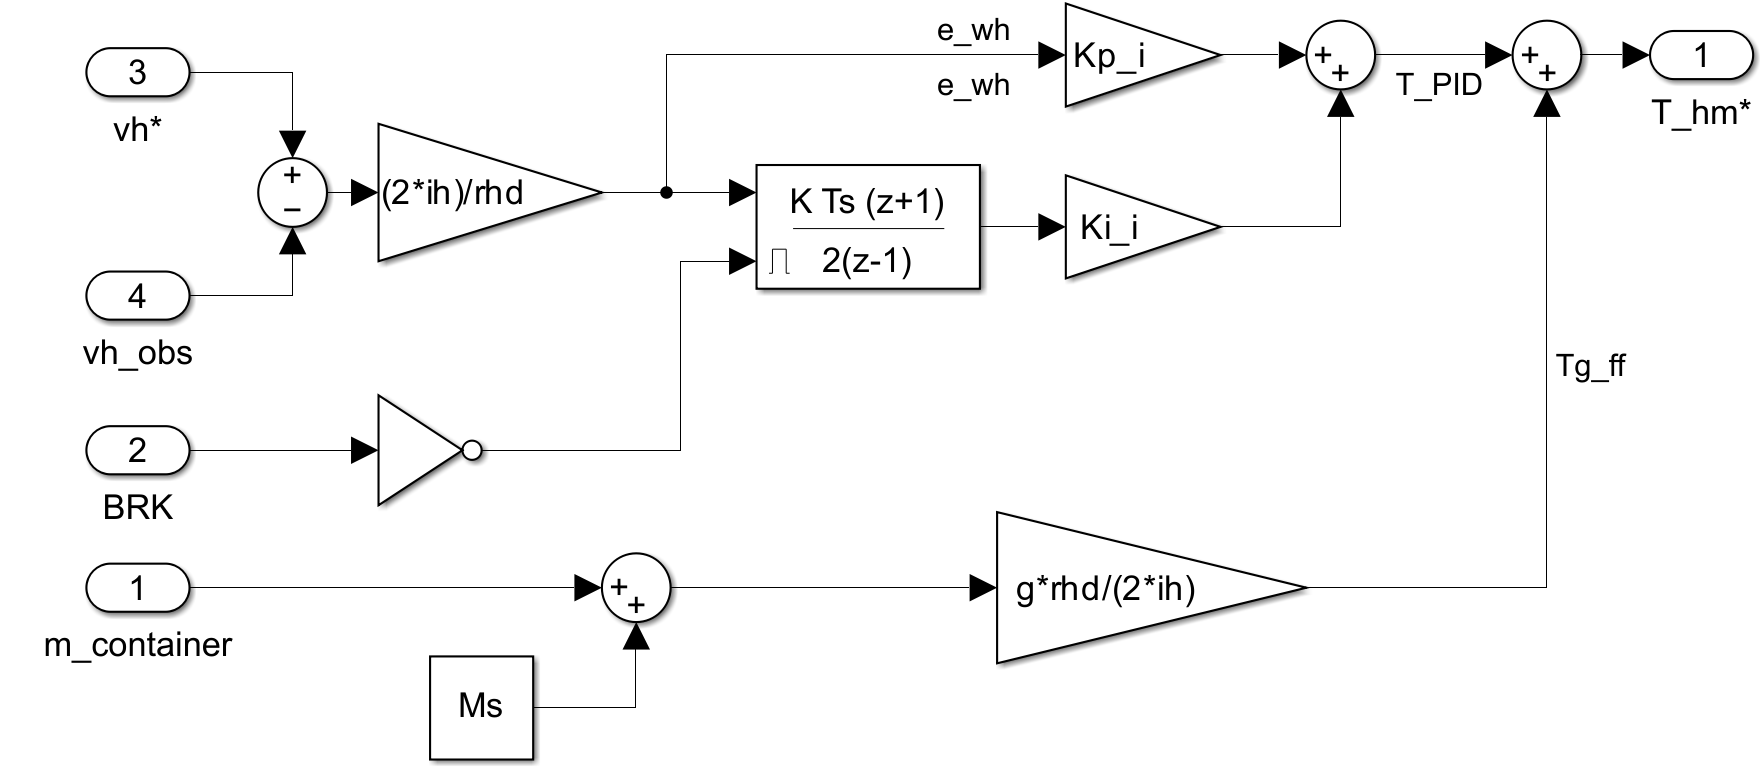
\includegraphics[width=0.72\linewidth]{nivel_2/lazo_controlador_izaje.png}
\end{frame}

\begin{frame}{Anti-windup y observador del izaje}
  \begin{columns}[T]
    \begin{column}{0.5\textwidth}
      \begin{block}{Anti-windup (dos frenos)}
        El izaje tiene freno de operación \sig{$BRK_h$} y de emergencia \sig{$BRK_{hE}$}:
        \textbf{cualquiera} de los dos resetea el integrador (igual criterio que el carro).
      \end{block}
    \end{column}
    \begin{column}{0.5\textwidth}
      \begin{block}{Observador con acción integral}
        Análogo al del carro, con las matrices del izaje. Ganancias por \textbf{separación de
        anchos de banda}: $\omega_{obs\,h} = 20\times$ el polo dominante de la planta, siendo $\omega_{obs\,h} = -9.5197\, rad/s$
      \end{block}
    \end{column}
  \end{columns}

  \vspace{0.3cm}
  \centering
  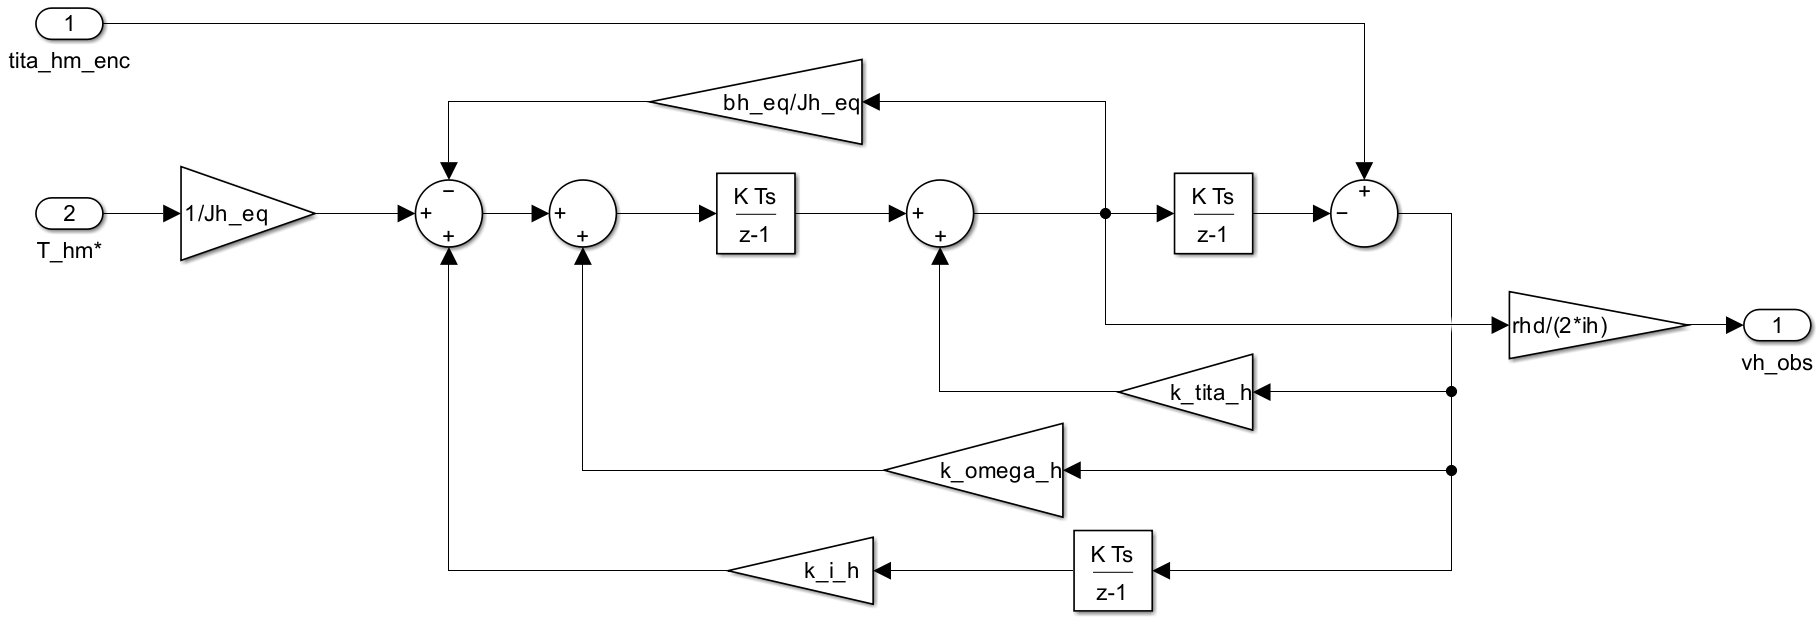
\includegraphics[width=0.78\linewidth]{nivel_2/obs_pid_izaje.png}
\end{frame}

\begin{frame}{Controlador regulatorio del carro (Simulink)}
  \centering
  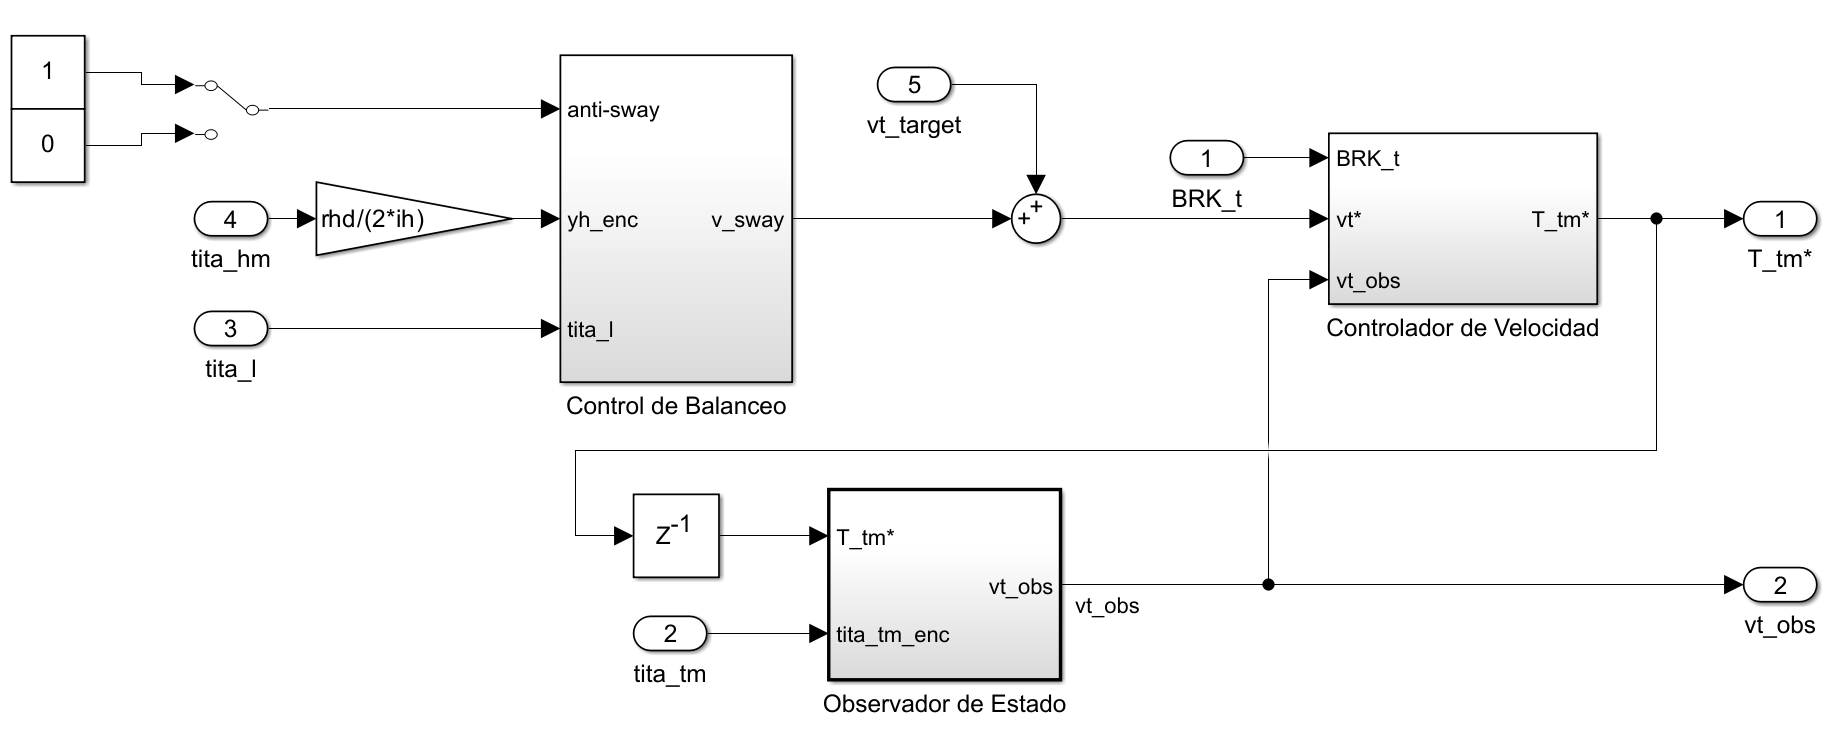
\includegraphics[width=\linewidth,height=0.82\textheight,keepaspectratio]{nivel_2/controlador_carro.png}
\end{frame}

\begin{frame}{Controlador regulatorio del izaje (Simulink)}
  \centering
  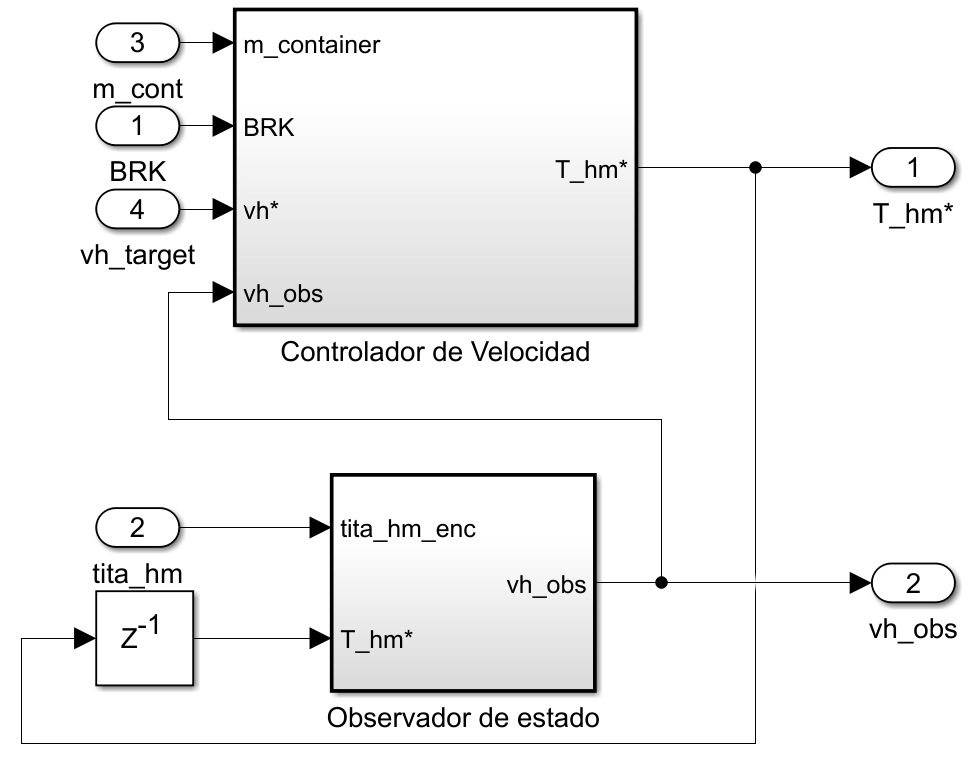
\includegraphics[width=\linewidth,height=0.82\textheight,keepaspectratio]{nivel_2/controlador_izaje.png}
\end{frame}
